% !TEX root = ../bachlor-arbeit.tex
\begin{tabular}{ll}
    \toprule
    Input: &
    \begin{tabular}[t]{@{}l@{}}
        transmission spectrum $I=(I_\s{x}, \,I_\s{y})$ a $\lambda \times 2$ array\\
        $I_\s{x/y}$ ... X- and Y-transmission spectra,
        $\lambda$ ... number of wavelengths
    \end{tabular}\\
    Output: &
    two sets layer parameters $\mc L_1$ and $\mc L_2$,
    stack parameters $\mc S$ \\
    \bottomrule
\end{tabular}

\paragraph{Network Architecture}
This module is a 1D Convolutional Neural Network instead of the basic Multi Layer Perceptron. It was chosen to utilize the translational invariance of ConvNets. For example the concept "peak" should be learned independent of its position in the spectrum. As described in section \ref{sec:NN_bg}, a ConvNet provides this functionality. Another constraint on the network architecture arises from the different kind of outputs.
Most of the outputs are continuous but the choices about material $m$ and geometry $g$ are discrete/categorical.
These need different activation functions $\sigma$ to reach the different value ranges. The continuous outputs are mostly bounded by physical constraints and $m, \, g \in [0, \, 1]$ as they are \textit{one hot encoded}, meaning $1 \rightarrow$ "The layer has this property" and
$0 \rightarrow$ "The layer does not have this property".


\indent The different outputs also need different cost functions $C(y, y')$ during training where $y'$ is the networks output and $y$ is the known solution. For the continuous output one can simply use the mean squared error
\begin{equation}
    C_\s{mse}(\vb y, \, \vb y') = \sum_i \qty(y_i - y_i')^2
\end{equation}

\noindent
as all outputs are equally important and the cost function should be indifferent on whether the networks prediction is over or under target. For the categorical output the network learns quicker with the \textit{Categorical Cross-Entropy} error

\begin{equation}
    C_\s{ce}(\vb y, \, \vb y') = - \sum_i y_i \log y'_i.
\end{equation}

\noindent
This error treats false positives ($y_i = 0, \, y_i' = 1$) and false negatives ($y_i = 1, \, y_i' = 0$) differently. A false positive does not increase the overall cost as $y_i = 0 \Rightarrow C_\s{ce} = 0$ but for a false negative $C_\s{ce} \rightarrow \infty$. This is favorable behavior because it does not matter if the network outputs some probability for a wrong class as long as it outputs a higher probability for the correct class. The final architecture, seen in figure \ref{fig:al:NN_architecture}, is similar to the example given in figure \ref{fig:bg:NN_example} while meeting the above-mentioned constraints.

\begin{figure}[H]
    \centering
    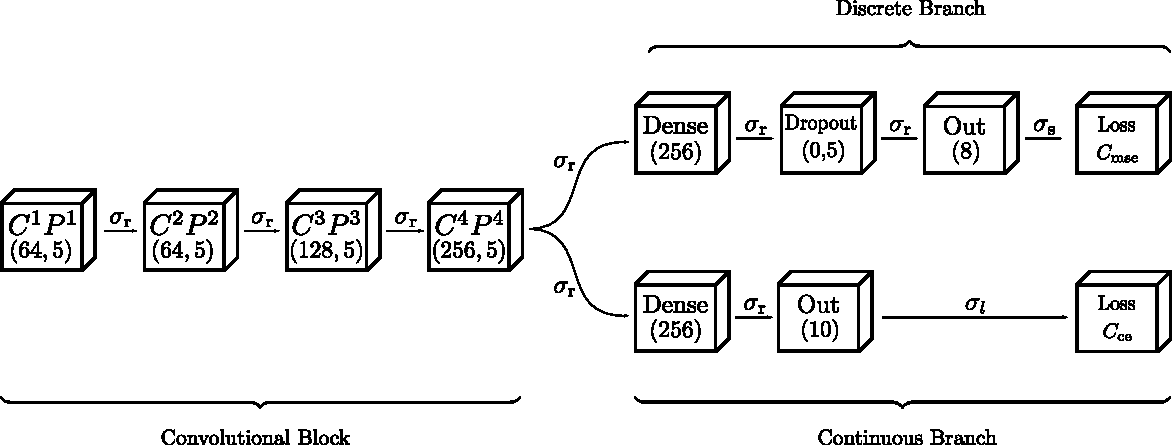
\includegraphics[width=\linewidth]{al_NN_architecture}
    \caption{The network starts with 4 pairs of convolutional and pooling layers $C^i P^i   $. The convolutions are characterized by (\textit{number of kernels}, \textit{kernel size}). The kernel size is always 5 and the number of kernels is gradually increased. Then the Network splits into a discrete and a continuous branch via two Dense layers with (\textit{number of neurons}). In the discrete branch a dropout is applied to the dense layer where (0.5) is (\textit{fraction of neurons to drop}).
    All the internal activations $\sigma_\s{r}$ are ReLu's and the final activations $\sigma_\s{s}$ and $\sigma_{l}$ are a sigmoid and a linear function.}
    \label{fig:al:NN_architecture}
\end{figure}

\newpage
\paragraph{Network Training}~\\
To train a Neural Network, one needs a training set $(X, \, Y)$ of known input output pairs. In this case they are generated using the pre-simulated single layers in the database which are randomly combined into stacks. Then the stacks X- and Y-transmission spectra $(I_x, \, I_y)$ are calculated via SASA.
This means $I = (I_x, \, I_y) \in X$ are the networks input and the random design parameters ${\mc D = (\mc S, \mc L_1, \mc L_2) \in Y}$ are the output. For the first test we used squares and square holes of Aluminum and Gold. During the training one epoch is defined as one loop over all training samples. After every epoch the network is validated on a data set $(X_\s v, \, Y_\s v)$ of samples it has not seen before. This is done to check wether the network actually learns something rather than just memorizing the input data.  The results of this first training on the square geometry can be seen in figure \ref{fig:al:square_results}.
\\

\indent
Training and validation results are very similar which indicates that there is no overfitting or memorization. The discrete accuracy quickly reaches a maximum of $\sim 76\%$ which is less than expected and also the speed at which this value is reached is suspicious. The network does not improve much after the fourth epoch and this does not change by tuning the network architecture. This is because the issue lies not within the architecture but in the training data. In section \ref{sec:SASA} we have shown that for the used two layer stacks the transmission spectrum is reciprocal, that is the same for both directions. Therefor the data generation can result in two different stacks which produce the same spectrum. Consider a stack where one layer is Aluminum and the other is Gold as seen in figure \ref{fig:al:same_spec}. As both of them produce the same spectrum, one time the network is taught that the first layer is Gold and the second is Aluminum but another time it is taught the complete opposite. Actually, if the network is trained this way it only ever predicts stacks with layers of equal materials because this is the only setup it can get right.

\begin{figure}[H]
    \centering
    \captionsetup[subfigure]{position=b}
    \begin{subfigure}{.5\textwidth}
        \centering
        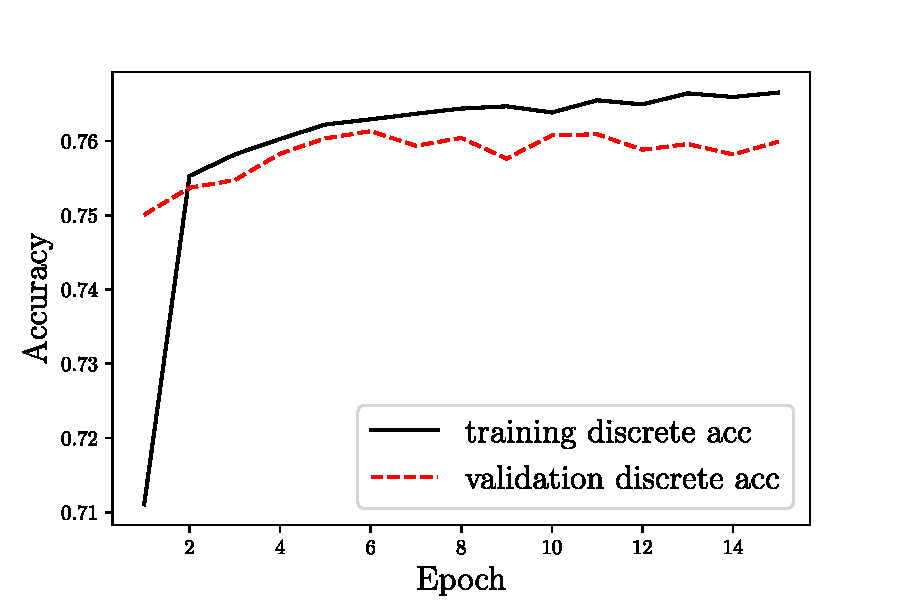
\includegraphics[width=\linewidth]{al_square_dis}
        \caption{}
    \end{subfigure}%
    \begin{subfigure}{.5\textwidth}
        \centering
        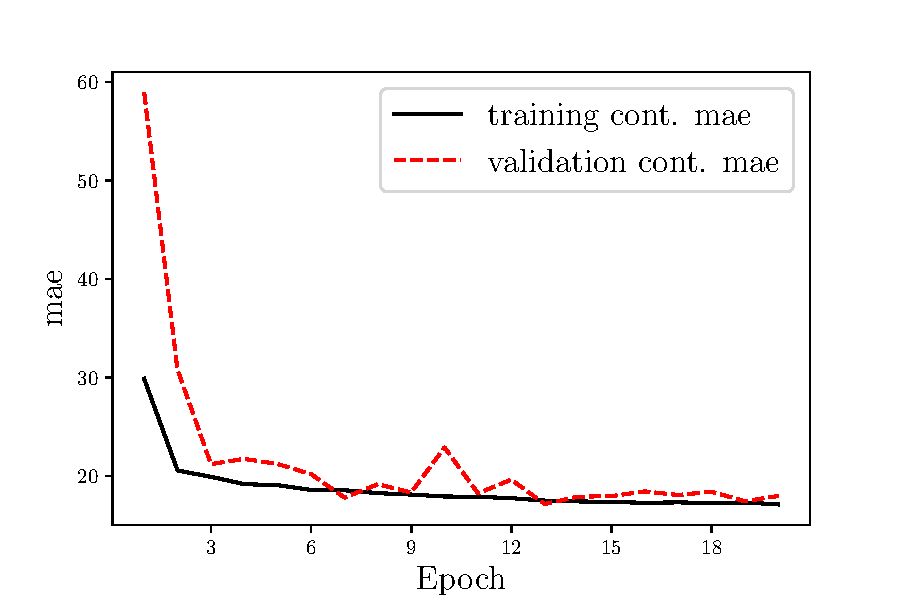
\includegraphics[width=\linewidth]{al_square_mae}
        \caption{}
    \end{subfigure}
    
    \caption{Training only with squares. (a) shows the accuracy of the discrete branch. That is, what percentage of choices for material and geometry were correct. In (b) we can see the performance of the continuous branch evaluated using the mean absolute error (mae).
    $C_\s{mae}(\vb y, \vb y') = \sum_i \qty|y_i - y'_i|$.}
    \label{fig:al:square_results}
    \end{figure}

\begin{figure}[H]
    \floatbox[{\capbeside\thisfloatsetup{capbesideposition={right,top}}}]{figure}[\FBwidth]
    {\caption{A stack of one Gold and one Aluminium layer separated by a glass spacer. Both stacks produce the same spectrum which leads to issues when using completely random stacks to train the network.}
    \label{fig:al:same_spec}}
    {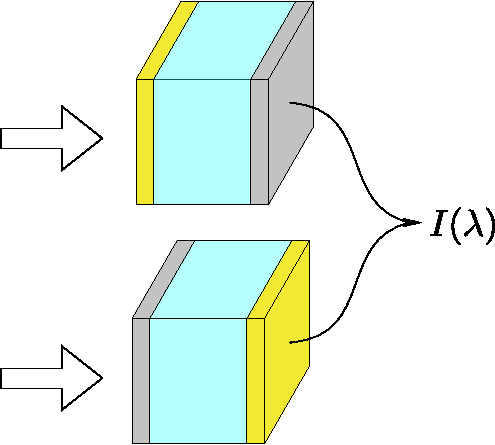
\includegraphics[width=.36\textwidth]{al_flipped_stack}}
\end{figure}


\newpage
This is a well known problem when trying to solve an inverse problem.
In this case the function $\mc D \rightarrow I$ is well defined as one stack can only produce one spectrum but for the inverse problem we are trying to solve $I \rightarrow \mc D$ and there might be multiple designs which produce the same spectrum. We can solve the issue simply by allowing only one of the orientations into the training data. By doing this the training  results change as seen in figure \ref{fig:al:squares_fix}.
\\

\indent
The discrete accuracy is much better at $\sim 98 \%$ and the training curve looks more natural in the sense that improvements diminish over time but do not hit a sudden barrier as they did in figure \ref{fig:al:square_results}.
Having resolved this issue, we can train the model on the more complex rectangle geometry reaching 94\% accuracy and 11 mae.


\begin{figure}[H]
\centering
\begin{subfigure}{.5\textwidth}
    \centering
    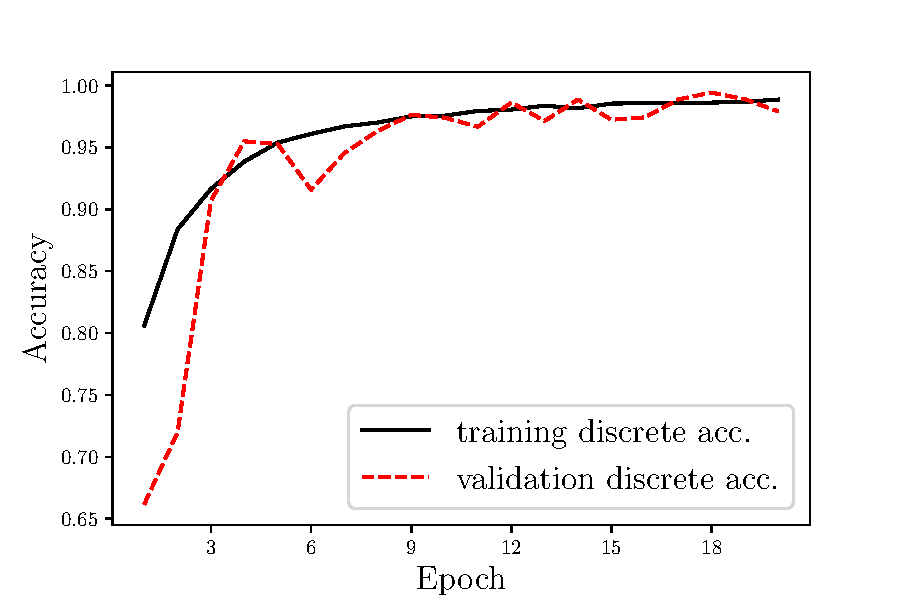
\includegraphics[width=\linewidth]{al_square_fix_dis}
    \caption{}
    \label{}
\end{subfigure}%
\begin{subfigure}{.5\textwidth}
    \centering
    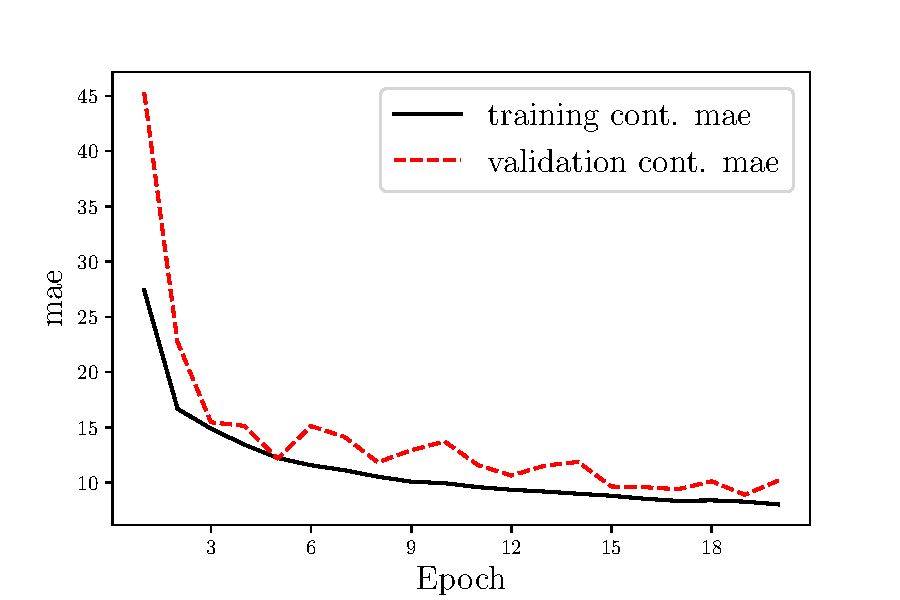
\includegraphics[width=\linewidth]{al_square_fix_mae}
    \caption{}
    \label{}
\end{subfigure}
\caption{Training on the square geometry after only allowing one of the equivalent stacks shown in figure \ref{fig:al:same_spec} into the training data.
Again, (a) shows the accuracy of the discrete branch and (b) the average cost of the continuous branch. The discrete accuracy has improved significantly compared to figure \ref{fig:al:square_results} but the continuous loss remains similar.}
\label{fig:al:squares_fix}
\end{figure}

